%!TEX root=../../autopilot.tex
\section{Reproducibility}
\label{sec:reproducibility}

We take a broad view on reproducibility: including not only the ability to share data and recreate experiments, but also integrating into a broader ecosystem of tools that reduces labor duplication and encourages sharing and organizing technical knowledge. For us, reproducibility means building a set of tools that make every experiment and every technique available to anyone, anywhere.

\subsection{Standardized task descriptions}

\begin{marginfigure}[-2cm]
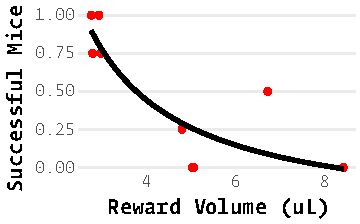
\includegraphics[width=\linewidth]{autopilot/autopilot/src/figures/calibration_warning.pdf}
\caption{\textbf{"Minor" details have major effects.} Proportion of mice (each point, n=4) that were successful learning the first stage of the speech task described in \citep{saundersMiceCanLearn2019} across 10 behavior boxes with variable reward sizes. A $2 \mu L$ difference in reward size had a surprisingly large effect on success rate.}
\label{fig:calibration}
\end{marginfigure}

The implementation and fine details of a behavioral experiment matter. Seemingly trivial details like milliseconds of delay between trial phases and microliters of reward volume can be the difference between a successful and unsuccessful task (Figure \ref{fig:calibration}). \textit{Reporting} those details can thus be the difference between a reproducible and unreproducible result.  Researchers also often use "auxiliary" logic in tasks---such as methods for correcting response bias---that are never completely neutral for the interpretation of results. These too can be easily omitted due to brevity or memory in plain-English descriptions of a task, such as those found in Methods sections. Even if all details of an experiment were faithfully reported, the balkanization of behavioral software into systems peculiar to each lab (or even to individuals within a lab) makes actually performing a replication of a behavior result expensive and technically challenging. Widespread use of experimental tools that are not explicitly designed to preserve every detail of their operation presents a formidable barrier to rigorous and reproducible science\citep{wallReliabilityStartsExperimental2019}.

%
%
%
Autopilot splits experiments into a) the \textbf{code} that runs the experiment, which is intended to be standardized and shared across implementations, and b) the \textbf{parameters} (Figure \ref{fig:params}) that define your particular experiment and system configuration. For example, two-alternative forced choice tasks have a shared structure regardless of the stimulus modality, but only your task plays pitch-shifted national anthems. This division of labor, combined with Autopilot's structured plugin system, help avoid the ubiquitous problem of rig-specific code and hard-coded variables making experimental code only useful on the single rig it was designed for --- enabling the possibility of a shared library of tasks as described in \hyperref[sec:expansion]{section \ref{sec:expansion}}%

\begin{marginfigure}[0cm]
\begin{minted}[frame=lines,fontsize=\small]{json}
{
"step_name"    : "tone_discrim",
"task_type"    : "2AFC",
"bias_mode"    : 0,
"punish_sound" : false,
"stim" : {
  "sounds" : {
    "L": {
      "duration"  : 100,
      "frequency" : 10000,
      "type"      : "tone",
      "amplitude" : 0.01},
    "R": {"...":"..."}}},
"reward": {
  "type"     : "volume",
  "volume"   : 20},
"graduation" : {
    "type"      : "accuracy",
    "threshold" : 0.75,
    "window"    : 400},
}
\end{minted}
\caption{Task parameters are stored as portable JSON, formatting has been abbreviated for clarity.}
\label{fig:params}
\end{marginfigure}%

The practice of reporting exactly the parameter description used by the software to run the experiment removes any chance for incompleteness in reporting. Because all task parameters are included in the produced data files, tasks are fully portable and can be reimplemented exactly by anyone that has comparable hardware to yours. 

\subsection{Self-Documenting Data}
\label{sec:data}

\begin{marginfigure}[1.5cm]
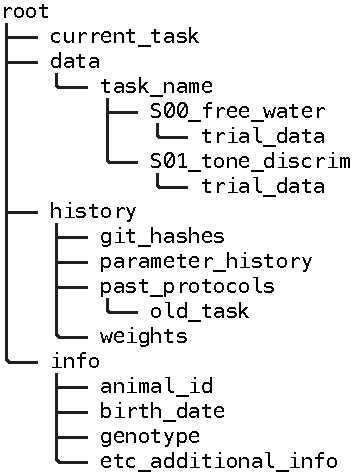
\includegraphics[width=\linewidth]{autopilot/autopilot/src/figures/side_16_data.pdf}
\caption{Example data structure. All information necessary to reconstruct an experiment is automatically stored in a human-readable HDF5 file.}
\label{fig:datastx}
\end{marginfigure}

A major goal of the open science movement is to normalize publishing well documented and clearly formatted data alongside every paper. Typically, data are acquired and stored in formats that are lab-idiosyncratic or ad-hoc, which, over time, sprout entire software libraries needed just to clean and analyze it. Idiosyncratic data formats hinder collaboration within and between labs as the same cleaning and analysis operations gain multiple, mututally incompatible implementations, duplicating labor and multiplying opportunities for difficult to diagnose bugs. Over time these data formats and their associated analysis libraries can mutate and become incompatible with prior versions, rendering years of work inaccessible or uninterpretable. In one worst-case scenario, the cleaning process unearths some critically missing information about the experiment, requiring awkward caveats in the Methods section or months of extra work redoing it. In another, the missing information or bugs in analysis code are never discovered, polluting scientific literature with inaccuracies. 

The best way to make data publishable is to avoid cleaning data altogether and \textit{design good data hygiene practices into the data acquisition process.} Autopilot automatically stores all the information required to fully reconstruct an experiment, including any changes in task parameters or code version that happen throughout training as the task is refined.

Autopilot data is stored in \href{https://support.hdfgroup.org/HDF5/whatishdf5.html}{HDF5} files, a hierarchical, high-performance file format. HDF5 files support metadata throughout the file hierarchy, allowing annotations to natively accompany data. Because HDF5 files can store nearly all commonly used data types, data from all collection modalities---trialwise behavioral data, continuous electrophysiological data, imaging data, etc.---can be stored together from the time of its acquisition. Data is always stored with the full conditions of its collection, and is ready to analyze and publish immediately (Figure \ref{fig:datastx}). No Autopilot-specific scripts are needed to import data into your analysis tool of choice---anything that can read HDF5 files can read Autopilot data\sidenote{Though our \texttt{Subject} class provides a simplified interface to access and manipulate Autopilot data}. 

As of v0.5.0, we have built a formal data modeling system into Autopilot, allowing for unified declaration of data for experimental subjects, task parameters, and resulting data with verifiable typing and human-readable annotations. These abstract data models can be used with multiple storage interfaces, paving the way for export to, for example, the Neurodata Without Borders standard\citep{rubelNWBAccessibleData2019}, further enabling Autopilot data to be immediately incorporated into existing processing pipelines (see section \ref{sec:datamodel}).

\subsection{Testing \& Continuous Integration}

Open-source scientific software does away with prior limitations to access and inspection imposed by proprietary tools. It also exposes the research process to bugs in software written by semi-amateurs that can yield errors in the resulting data, analysis, and interpretation\citep{soergelRampantSoftwareErrors2015,eklundClusterFailureWhy2016a,bhandarineupaneCharacterizationLeptazolinesPolar2019,millerScientistNightmareSoftware2006}. Autopilot tries to bring best practices in software development to experimental software, including a set of automated tests for continuous integration. 

We are still formalizing our contribution process, and our tests are still far from achieving full coverage\sidenote{Coverage statistics for Autopilot are available on coveralls.io at \url{https://coveralls.io/github/auto-pi-lot/autopilot}}, but we currently require tests and documentation for all new code added to the library. Writing good tests is hard, and we are in the process of building a set of hardware simulators and test fixtures to ease contribution.  

Tests are effectively provable statements about how a program functions (Figure \ref{fig:tests}), which are particularly important for a library that aspires to be baseline lab infrastructure like Autopilot. Tests make it possible to use and contribute to the library with confidence: all tests are run on every commit, making it possible to determine if some new contribution breaks existing code without manually reading and testing every line. As we work to complete our test coverage, we hope to provide researchers with a tool that they can trust and elevates the verifiability of scientific results at large.

\begin{marginfigure}[-0cm]
\begin{minted}[frame=lines,fontsize=\small]{python}
def test_set_gpio():
    """
    The `set` method of a Digital_Out
    object sets the pin state
    """
    pin = Digital_Out(pin=17)

    # Turn GPIO pin on
    pin.set(True)
    assert pin.state == True

    # Turn GPIO pin off
    pin.set(False)
    assert pin.state == False
\end{minted}
\caption{A test like \texttt{test\_set\_gpio} is a provable statement about the functionality of a program, in this case that "the \texttt{Digital\_Out.set()} method sets the state of a GPIO pin."}
\label{fig:tests}
\end{marginfigure}

\subsection{Expense}
\label{sec:expense}

Autopilot is an order of magnitude less expensive than comparable behavioral systems (Table \ref{tab:cost}). We think the expense of a system is important for two reasons: scientific equity and statistical power. 

The distribution of scientific funding is highly skewed, with a large proportion of research funding concentrated in relatively few labs\citep{katzBiomedicalEliteInequality2017}. Lower research costs benefit all scientists, but lower instrumentation costs directly increase the accessibility of state-of-the-art experiments to labs with less funding. Since well-funded labs also tend to be concentrated at a few (well-funded) institutions, lower research costs also broaden the base of scientists outside traditional research institutions that can stay at the cutting edge\citep{ashkenasEvenAffirmativeAction2017,clausetSystematicInequalityHierarchy2015,pearceExpandingEquitableAccess2019}.
%
\begin{marginfigure}[0.5cm]
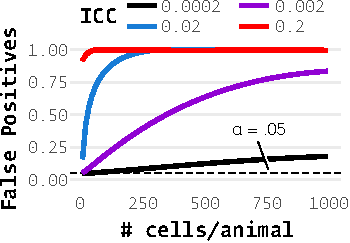
\includegraphics[width=\linewidth]{autopilot/autopilot/src/figures/fpr.pdf}
\caption{When comparing a value across groups, eg. a genetic knockout vs. wildtype, even a modest intra-animal (or, more generally, intra-cluster) correlation (ICC) causes the false positive rate to be far above the nominal $\alpha = 0.05$. Shown are false positive rates for simulated data with various numbers of "cells" recorded for comparisons between two groups of 5 animals each with a real effect size of 0. We note that 741 simultaneously recorded cells were reported in \citep{junFullyIntegratedSilicon2017} and a mean ICC of 0.19 across 18 neuroscientific datasets was reported in \citep{aartsSolutionDependencyUsing2014}}
\label{fig:icc}
\end{marginfigure}%
%
Neuroscience also stands to benefit from the lessons learned from the replication crisis in Psychology\citep{shroutPsychologyScienceKnowledge2018}. In neuroscience, underpowered experiments are the rule, rather than the exception\citep{buttonPowerFailureWhy2013}. Statistical power in neuroscience is arguably even worse than it appears, because large numbers of observations (eg. neural recordings) from a small number of animals are typically pooled, ignoring the nested structure of observations collected within individual animals. Increasing the number of cells recorded from a small number of animals dramatically increases the likelihood of Type I errors (Figure \ref{fig:icc})---indeed, for values of within-animal correlation typical of neuroscientific data, high numbers of observations make Type I errors more likely than not\citep{aartsSolutionDependencyUsing2014}. For this reason, perhaps paradoxically, recent technical advances in multiphoton imaging and silicon-probe recordings will actually make statistical rigor in neuroscience \textit{worse} if we don't use analyses that account for the multilevel structure of the data and correspondingly record from the increased number of animals that they require.




Although the expense of multi-photon imaging and high-density electrophysiology will always impose an experimental bottleneck, behavioral training time is often the greater determinant of study sample size. Typical behavioral experiments require daily training sessions often carried out over weeks and months, while far fewer imaging or electrophysiology sessions are carried out per animal.  Training large cohorts of animals in parallel is thus the necessary basis of a well-powered imaging or electrophysiology experiment.


\begin{table}[hb!]
\caption{\textbf{Cost for Basic 2AFC System}\\
\noindent"Nosepoke" includes a solenoid valve, IR sensor, water tube, LED, housing, and any necessary driver PCBs. For PyControl and Autopilot, we included the cost of one \href{https://wiki.auto-pi-lot.com/index.php/Lee_LHDA0531115H}{Lee LHDA0531115H} solenoid valve per nosepoke (\$63.35). For PyControl, we estimated a typical USB hub with 5 ports to control 5 pyControl systems from one computer. We note that the Bpod and PyControl systems both include cost of assembly for the control CPUs and nosepokes, but also that Autopilot does not require assembly for its control CPU and its default nosepoke is a snap-together 3D printed part and PCB without surface mounted components that can be assembled by an amateur in roughly half an hour.}
\label{tab:cost}
\noindent\begin{tabularx}{\linewidth}{XRRR}\toprule
& Autopilot & pyControl & Bpod  \\
\midrule
Behavior CPU & 
\href{https://www.adafruit.com/product/4292}{\texttt{\$45}} & 
\href{https://open-ephys.org/pycontrol/pycontrol}{\texttt{\$270}} & 
\href{https://sanworks.io/shop/viewproduct?productID=1024}{\texttt{\$925}}\\
Nosepoke (3x) & 
\texttt{\$216} & 
\href{http://www.open-ephys.org/store/pycontrol-peripherals}{\texttt{\$369}} & 
\href{https://sanworks.io/shop/viewproduct?productID=1009}{\texttt{\$810}} \\
\textbf{Total for One} & 
\textbf{\texttt{\$261}} & 
\textbf{\texttt{\$639}} & 
\textbf{\texttt{\$1735}}\\
\midrule
Five Systems & 
\texttt{\$1305} & 
\texttt{\$3195} & 
\texttt{\$8675} \\
Host CPU(s) & 
\texttt{\$1000} & 
\texttt{\$1000} & 
\texttt{\$5000} \\
\textbf{Total for Five} & 
\textbf{\texttt{\$2305}} & 
\textbf{\texttt{\$4195}} & 
\textbf{\texttt{\$13625}} \\
\midrule
\textbf{Total for Ten} & 
\textbf{\texttt{\$3610}} & 
\textbf{\texttt{\$8390}} & 
\textbf{\texttt{\$27350}} \\
\bottomrule
\end{tabularx}
\end{table}
